\chapter{Generative models in anomaly detection} \label{sec:chapter_survey}
Suppose that a given problem (e.g. classification) is requires us to model some directly observable data, denoted by $\vc{x}$, which is somehow connected with a second variable $\vc{z}$, which might not be directly observable, or we only have a finite set of observed pairs $(\vc{x},\vc{z})$. When $\vc{z}$ is discrete, it has the interpretation of a \textbf{label} which denotes an affiliation with one of a finite number of classes (in that case, it is often denoted by $\vc{y}$ instead). When it is continuous, we use the term \textbf{hidden} or \textbf{latent} variable, see Sec.~\ref{sec:probabilistic_models}, where it was already discussed. In that case, we assume that there is some mechanism that connects $\vc{x}$ and $\vc{z}$ that can be modeled e.g. by a decoder $g_{\vc{\theta}}(z)$ from Sec.~\ref{sec:reconstruction_models}. The term \textbf{generative model} denotes an approach when the joint probability distribution of $p(\vc{x},\vc{z})$ is modeled, as opposed to a \textbf{discriminative model}, which tries to estimate $p(\vc{z} \vert \vc{x})$. An example of a discriminative model is a logistic classifier, which in fact estimates $p(\vc{z} \vert \vc{x})$ as a function $f:\mathcal{X} \rightarrow \mathcal{Z}$ where $\mathcal{Z} = [0,1]$, i.e. it produces a guess for binary label based on input data. While it seems that a generative model is more flexible, as it can provide  $p(\vc{z} \vert \vc{x}) = p(\vc{x},\vc{z})/p(\vc{x})$, it is usually subpar in classification tasks~\cite{ng2001discriminative,bishop2007generative}. The advantage of using a generative model is that it can generate artificial samples $\vc{x}$, and most importantly, it can be trained in an unsupervised manner (without observed labels/latent variables) and provide an estimate of the data distribution $p(x)$. This is the reason generative models are interesting for anomaly detection, together with the advent of deep generative models that can model large quantities of high-dimensional data.

Some generative models were actually already introduced in the previous chapter in Sec.~\ref{sec:probabilistic_models}, such as the Gaussian Mixture Model, autoregressive models or various energy based models. Recently, very large deep generative models with billions of parameters were introduced. They are pushing the boundaries in many domains and produce human-like outputs, such as the BigGAN~\cite{brock2018large} for images, GPT-3~\cite{brown2020language} for text, the Jukebox model~\cite{dhariwal2020jukebox} for music generation, or diffusion models~\cite{sohl2015deep} for text-to-image translation~\cite{saharia2022photorealistic}. In the previous chapter, we have already mentioned the three main types of deep generative models that will be discussed in greater depth in this chapter -- the \textbf{Generative Adversarial Network} (GAN)~\cite{goodfellow2014gan}, the \textbf{Variational Autoencoder} (VAE)~\cite{kingma2013vae} and various \textbf{flow models}~\cite{dinh2014nice}. They present the basic paradigms on which most of novel anomaly detectors are built~\cite{an2015variational,xu2018unsupervised,wang2018generative,perera2019ocgan,yamaguchi2019adaflow,schmidtNormalizingFlowsNovelty2019}. 

\section{GAN--based models} \label{sec:gan_models}
The \textbf{Generative Adversarial Network} (GAN) was introduced in~\cite{goodfellow2014gan} where it was successfully used to generate MNIST digits, faces and CIFAR-10 images. Since then, GAN-based models were used in a multitude of different areas, such as next frame prediction in videos~\cite{lotter2015unsupervised}, semi--supervised learning~\cite{salimans2016fmgan}, image--to--image translation~\cite{zhu2016generative}, semantic manipulation of high resolution images~\cite{wang2018high} or for generating realistic artificial image~\cite{karras2019style} and audio data~\cite{lee2022bigvgan}. In comparison with VAE-based generative models, it is believed that GAN-based models produce pictures that are more realistic (less blurry), at the cost of difficult and highly unstable training~\cite{salimans2016fmgan}. In the following text, the basics of GANs will be introduced together with their applications to anomaly detection. 

\subsection{Basic GAN model}
\begin{figure}
\centering{}\begin{tikzpicture}
  % code
  \node[const]           (z) {$\vc{z} \sim p(\vc{z})$};
  \node[const, right = 0.3cm of z]           (zin) {};
  % decoder in
  \node[latent, right = 0.4cm of z, yshift = 0.275cm] (G11) {};
  \node[latent, right = 0.4cm of z, yshift = -0.275cm] (G12) {};
  % decoder hidden
  \node[latent, right = 1.6cm of z, yshift = 0.55cm] (G21) {};
  \node[latent, right = 1.6cm of z, yshift = 0cm] (G22) {};
  \node[latent, right = 1.6cm of z, yshift = -0.55cm] (G23) {};
  % decoder out
  \node[latent, right = 2.8cm of z, yshift = 0.825cm] (G31) {};
  \node[latent, right = 2.8cm of z, yshift = 0.275cm] (G32) {};
  \node[latent, right = 2.8cm of z, yshift = -0.275cm] (G33) {};
  \node[latent, right = 2.8cm of z, yshift = -0.825cm] (G34) {};
  % generator tag
  \node[const, right = 1.6cm of z, yshift = 1.1cm] (G) {$g_{\vc{\theta}}(\vc{z})$};
  % x
  \node[const, right = 4.0cm of z]           (xg) {$\tilde{\vc{x}}$};
  \node[const, right = -0.8cm of xg]          (xout) {};
  \node[const, right = 0.5cm of xg]           (xin) {};
  \node[const, right = -0.7cm of xg, yshift=1.3cm]      (x) {$\vc{x} \sim p(\vc{x})$};
  \node[const, right = -0.05cm of xg, yshift=1.1cm]      (xpout) {};
  \node[const, right = 0.5cm of xg, yshift=0.1cm]      (xpin) {};
  % encoder in
  \node[latent, right = 0.7cm of xg, yshift = 0.825cm] (D11) {};
  \node[latent, right = 0.7cm of xg, yshift = 0.275cm] (D12) {};
  \node[latent, right = 0.7cm of xg, yshift = -0.275cm] (D13) {};
  \node[latent, right = 0.7cm of xg, yshift = -0.825cm] (D14) {};
  % encoder hidden
  \node[latent, right = 1.9cm of xg, yshift = 0.55cm] (D21) {};
  \node[latent, right = 1.9cm of xg, yshift = 0cm] (D22) {};
  \node[latent, right = 1.9cm of xg, yshift = -0.55cm] (D23) {};
  % encoder out
  \node[latent, right = 3.1cm of xg, yshift = 0cm] (D31) {};
  % xhat
  \node[const, right = 4.1cm of xg]           (dx) {$s_d \in [0,1]$};
  \node[const, right = -1.9cm of dx]       (dxout) {};       
  % discriminator tag
  \node[const, right = 1.9cm of xg, yshift = 1.1cm] (D) {$d_{\vc{\varphi}}(\vc{x})$};
  
  % edges
  % latent
  \nedge {z} {zin}
  % generator
  \nedge {G11, G12} {G21, G22, G23}
  \nedge {G21, G22, G23} {G31, G32, G33, G34} 
  
  % x 
  \nedge {xout} {xg}
  \nedge {xg} {xin}
  \nedge {xpout} {xpin}
  % discriminator
  \nedge {D11, D12, D13, D14} {D21, D22, D23}
  \nedge {D21, D22, D23} {D31}
  %xhat
  \nedge {dxout} {dx}
\end{tikzpicture}
\caption{A schematic of a GAN consisting of fully connected layers. A latent
noise sample $\vc{z}\sim p(\vc{z})$ is fed to the generator $g_{\vc{\theta}}(\vc{z})$
which then produces an artificial sample $\tilde{\vc{x}}$. Alternatively,
a sample $\vc{x}$ is sampled from the data distribution $p(\vc{x})$. Both
are passed to the discriminator $d_{\vc{\varphi}}(\vc{x})$ that produces a score
$s_d$ -- the probability that $\tilde{\vc{x}}$ or $\vc{x}$ come from the
true data distribution.}
\label{fig:gan}
\end{figure}

Suppose that we have samples from the true data distribution $p(\vc{x}),\vc{x}\in\mathcal{X}$, which we are trying to imitate. We don't know the true form of $p(\vc{x})$, since it is usually high-dimensional and not representable directly by a function, but instead it is available to us through a finite set of samples that comprise the training dataset $X = \lbrace \vc{x}_1, \vc{x}_2, \ldots, \vc{x}_n \rbrace \subset \mathcal{X}$. The goal is to build a proxy for $p(\vc{x})$ so that we can draw new, yet unseen samples from it. The GAN tackles this problem by a model with two principal parts. First is the \textbf{generator}, which is a neural network that represents a mapping $g_{\vc{\theta}}(\vc{z}):\mathcal{Z}\rightarrow\mathcal{X}$, where $\vc{\theta}$ are its weights, and $\mathcal{Z}$ is the latent space. Note that we use the same notation for the generator that was already used for a decoder in the AE model -- this is because they fulfill the same role in both models. We will denote a generated sample by $\tilde{\vc{x}} = g_{\vc{\theta}}(\vc{z})$. Since the generator as we have defined it so far is deterministic and we need to cover a random distribution, the inputs to the generator come from a \textbf{prior} noise distribution $p(\vc{z})$. The prior is usually chosen such that it it easy to generate samples from it, e.g. $p(\vc{z}) = \mathcal{N}(0,\vc{I})$, in which case $\mathcal{Z} = \mathbb{R}^h$ with $h$ being the dimension of the latent space. Then, the task is to train the generator in such a fashion that it learns the potentially highly non--linear mapping from $p(\vc{z})$ to $p(\vc{x})$. This is stimulated by the adversary of the generator -- the \textbf{discriminator}. We define it as a neural network with weights $\vc{\theta}$, i.e. a mapping $d_{\vc{\varphi}}(\vc{x}):\mathcal{X}\rightarrow\left[0,1\right]$. The output of the discriminator has the interpretation of the probability that its input comes from $p(\vc{x})$ rather than being generated by the generator, in other words, true samples $\vc{x}$ should be given higher value than the generated samples $\tilde{\vc{x}}$.

Both parts of a GAN are trained (their weights are updated) in tandem, so each of them iteratively improves in its task. The discriminator is trained both with true and generated samples to maximize the probability of assigning the correct label to them, while the generator is minimizing the probability of the discriminator recognizing the generated sample. This can be written down as a two player minimax~\cite{maschler2020game} game 
\begin{equation} \label{eq:gan_obj}
\min_{\vc{\theta}}\max_{\vc{\varphi}}\mathbb{E}_{ \vc{x} \sim p(\vc{x})}\left[\ln d_{\vc{\varphi}}(\vc{x})\right]+\mathbb{E}_{\vc{z}\sim p(\vc{z})}\left[\ln\left(1-d_{\vc{\varphi}}(g_{\vc{\theta}}(\vc{z}))\right)\right].
\end{equation}
It can be shown~\cite{goodfellow2014gan} that this objective has a saddle point at at $-\ln4$. In practice, \eqref{eq:gan_obj} is not used directly. That is because the term $\ln\left(1-d_{\vc{\varphi}}(g_{\vc{\theta}}(\vc{z}))\right)$ suffers from vanishing gradients -- when the generated samples do not resemble the real data in the beginning of the training, than this terms is almost zero and the generator is not trained. Therefore, instead of minimizing this, we can maximize $\ln d_{\vc{\varphi}}(g_{\vc{\theta}}(\vc{z}))$ to train the generator, which has much stronger gradients~\cite{goodfellow2014gan}. During training, we sample $\vc{x}$ from the training dataset and $\vc{z}$ from the prior distribution and update the generator and discriminator weights by minimizing
\begin{equation}\label{eq:gen_loss}
\mathcal{L}_{g}(\vc{z},\vc{\theta})= - \ln d_{\vc{\varphi}}(g_{\vc{\theta}}(\vc{z})),
\end{equation}
\begin{equation}\label{eq:disc_loss}
\mathcal{L}_{d}(\vc{x},\vc{z},\vc{\varphi})= - \ln d_{\vc{\varphi}}(\vc{x}) - \ln\left(1-d_{\vc{\varphi}}(g_{\vc{\theta}}(\vc{z}))\right).
\end{equation}
Note that we explicitly remove the dependency of the loss functions on the weights that are not being optimized through them. A detailed training procedure of a GAN is described in Alg.~\ref{alg:gan_train}. Interestingly, during training, the generator never encounters any sample coming from $p(x)$ but is still able to eventually learn the shape of $p(\vc{x})$. The choice of $p(\vc{z})$ can be rather arbitrary as far as sampling from it is possible and the generator and discriminator have sufficient capacity to process it. In practice, uniform or normal distribution is usually used, as already mentioned. 

\begin{algorithm}
\begin{algorithmic}[1]
\Require{Generator $g_{\vc{\theta}}$, discriminator $e_{\vc{\phi}}$, a training set $X=\lbrace \vc{x}_1, \vc{x}_2, \ldots, \vc{x}_n \rbrace \subset \mathcal{X}$, maximum number of iterations $I\in\mathbb{N}$, batchsize $L \in \mathbb{N}$.}
\State $\vc{\theta}, \vc{\varphi} \gets $ Initialize weights
\State{$i \gets $ Iteration counter}
\While{$i<I$ or $\vc{\theta}, \vc{\varphi}$ are not converged}
	\State{$X_L \gets$ A random batch of $L$ samples from $X$}
	\State{$Z_L \gets$ A random batch of $L$ samples from $p(\vc{z})$}
	\State$l_d \gets \frac{1}{L}\sum_{j=1}^L \mathcal{L}_d(\vc{x}_j,\vc{z}_j,\vc{\varphi}), \vc{x}_j \in X_L, \vc{z}_j \in Z_L$
	\State$\vc{\varphi} \stackrel{+}\gets - \nabla_{\vc{\varphi}} l_d$ update of discriminator weights 
	\State$l_g \gets \frac{1}{L}\sum_{j=1}^L \mathcal{L}_g (\vc{z}_j,\vc{\theta}), \vc{z}_j \in Z_L$
	\State$\vc{\theta} \stackrel{+}\gets - \nabla_{\vc{\theta}} l_g$ update of generator weights
	\State{$i \gets i+1$}
\EndWhile
\State{\textbf{return} generator $g_{\vc{\theta}}(\vc{z})$, discriminator $d_{\vc{\varphi}}(\vc{x})$}
\end{algorithmic}
\caption{GAN training procedure.}
\label{alg:gan_train}
\end{algorithm}

Achieving convergence such that the generated samples $\tilde{\vc{x}}$ resemble the training data might be difficult and require multiple random initializations of the model weights. Details on stable training of GANs can be found e.g. in~\cite{gui2021review}. A phenomenon called \textbf{mode collapse} has been described~\cite{goodfellow2016nips}, which happens when $p(\vc{x})$ is multimodal, but the generator distribution collapses to a single mode. A generator that has collapsed to a single mode of a MNIST dataset will produce only a single digit, e.g. "1", no matter where the code is sampled from. To mitigate this issue, several practices have been proposed~\cite{salimans2016fmgan,hong2019generative}. One of them is the use of an enhanced generator loss
\begin{equation} \label{eq:fmgan}
\mathcal{L}_{\text{gfm}}(\vc{z},\vc{x},\vc{\theta})=\alpha\mathcal{L}_{g}(\vc{z},\vc{\theta})+\mathcal{L}_{h}(\vc{z},\vc{x},\vc{\theta}),
\end{equation}
where the second term is the so-called \textbf{feature-matching} loss
\begin{equation} \label{eq:fm_loss}
\mathcal{L}_{fm}(\vc{z},\vc{x},\vc{\theta}) = ||d_{l,\vc{\varphi}}(\vc{x})-d_{l,\vc{\varphi}}(g_{\vc{\theta}}(\vc{z}))||_{2}^{2}
\end{equation}
where $\alpha > 0$ is a tunable weight and $d_{l,\vc{\varphi}}(\vc{x})$ is the intermediate representation of $\vc{x}$ after propagation through $l \in \mathbb{N}$ layers of the discriminator. This loss is supposed to provide improved gradients for the generator to stabilize the training. In the following text, a GAN model with the loss~(\ref{eq:fmgan}) will be referred to as the \textbf{feature-matching GAN} (fmGAN).

\subsection{GANs in anomaly detection}
The idea of using a GAN for anomaly detection comes from the the ability of the generator to learn the true data distribution $p(\vc{x})$ and especially the ability of the discriminator to recognize samples coming from $p(\vc{x})$. When the training dataset consists of normal samples, the discriminator output can be converted into an anomaly score
\begin{equation} \label{eq:disc_score}
     s_{\text{GAN}}(\vc{x}) = 1 - d_{\vc{\varphi}}(\vc{x}),
\end{equation}
which is higher for suspected anomalies and lower for normal data. The common critique is that the discriminator was not trained to recognize an arbitrary distribution of the anomalies but only that of the latent transformed by the generator. Thus it may fail to recognize anomalous samples of interest. 

The authors of the \textbf{AnoGAN} model~\cite{schlegl2017unsupervised} recognize this flaw. Their convolutional GAN model is trained with the feature-matching loss~\eqref{eq:fmgan}. For identification of anomalies in medical images, instead of using~\eqref{eq:disc_score}, they propose an iterative procedure that searches for the latent code $\vc{z}$ most likely to generate the tested sample to identify anomalous images. However, this procedure is computationally expensive. Therefore, an update to this model was published, the \textbf{f(ast)AnoGAN}~\cite{schleglFAnoGANFastUnsupervised2019}. It uses a Wasserstein GAN~\cite{gulrajani2017improved,haloui2018anomaly} (more on Wasserstein optimization objective in the next section) with gradient penalization~\cite{gulrajani2017improved} to improve training stability and adds an encoder distribution $q_{\phi}(\vc{z}|\vc{x})$ to find $\vc{z}$ closest to given $\vc{x}$ faster. The anomaly score of fAnoGAN is a combination of the discriminator score~\eqref{eq:disc_score} and the feature-matching loss~\eqref{eq:fm_loss}. 

The fmGAN model is used the publication~\cite{kliger2018novelty}, where it is tested on benchmark datasets such as MNIST and CIFAR-10. In~\cite{wang2018generative}, a GAN model was used to detect anomalies in time series data coming from industrial processes, whereas in~\cite{zenatiEfficientGANBasedAnomaly2018}, network intrusions were detected. In the \textbf{Multiple-Objective Generative Adversarial Active Learning} (MOGAAL)~\cite{liu2019generative}, $k \in \mathbb{N}$ generators are trained against a single discriminator on input data divided into $k$ subsets. The discriminator score Eq.~\eqref{eq:disc_score} is used to test new samples. The authors of~\cite{perera2019ocgan} claim to have achieved state-of-the-art results in one-class classification through severely restricting the latent space of the
GAN combined with an autoencoder and employing an adversarial data augmentation strategy. 

The use of GAN with an encoder~\cite{donahue2016adversarial} or an autoencoder with a discriminator~\cite{leveau2017adversarial} for anomaly detection is often and somehow blurs the line between GAN and VAE-based models, but we believe that presenting both concepts separately is useful. True GAN-like models for anomaly detection are however far less prevalent than models that use some autoencoding structure, which will be the focus of the next section. Experimental comparison of both approaches is presented in Chapter~\ref{sec:chapter_comparison}.

\section{VAE-based models} \label{sec:vae_models}
The \textbf{Variational Autoencoder} (VAE) is a generative model that has enjoyed a great success in a number of fields since its introduction in~\cite{kingma2013vae}. Its basic architecture~\cite{kingma2019introduction} is very similar to that of an AE model described in Sec.~\ref{sec:reconstruction_models}, but that is where the similarities end, as VAE is more of a probabilistic anomaly detector, since it models the probability distribution of the normal data. Unlike in AE, where the encoding to latent space $\mathcal{Z}$ is not constrained from taking any shape or form as far as the learning objective is minimized, in VAE a desired distribution of the encodings is explicitly prescribed in the form of a prior distribution $p(\vc{z})$. If the network is trained properly and the encodings follow the prior, we can feed samples from $p(\vc{z})$ to the decoder and expect to obtain random samples in the $\mathcal{X}$ space that will resemble those from the training dataset. This is the simple principle of how VAE works --- more details will be given in the following text.

The VAE has been mainly used for generation of artificial images such as faces~\cite{rezende2014stochastic} or sentences~\cite{bowman2015generating}, but also for other tasks such as semi--supervised learning~\cite{kingma2014semi}, segmentation~\cite{sohn2015learning}, static image forecasting~\cite{walker2016uncertain} and of course for anomaly detection~\cite{an2015variational,xu2018unsupervised,solch2016variational}. Since its popularity, a multitude of approaches enhancing the original VAE has been published, approaching the paradigm from different angles, with some of the more prominent examples published in~\cite{higgins2017beta,zhao2017infovae,tolstikhin2017wasserstein,makhzani2015adversarial,pu2017adversarial}. In the following text, we will go through the basic theory, its implications for the basic VAE, and through some of the extensions. 

\subsection{Basic VAE} \label{sec:vanilla_vae}
We will begin by defining the VAE from a probabilistic perspective. Let us assume that there is a dataset $X$ consisting of i.i.d samples. We want to obtain a tractable estimate of the true data distribution $p(\vc{x})$ in order to be able to sample from it. For that purpose, suppose that there is a hidden random process that generates the data and which involves a latent variable $\vc{z}$. Then, like in the case of the GAN model, we can redirect the sampling from the data space $\mathcal{X}$ to the latent space
$\mathcal{Z}$, in which it might be easier. Specifically, we want to sample from the latent prior distribution specified by a density $p(\vc{z})$, then pass this sample to the generative distribution with density $p_{\vc{\theta}}(\vc{x}|\vc{z})$, where $\vc{\theta}$ are its parameters, and obtain a sample $\vc{x}$ that will be very similar to the samples coming from the true data distribution $p(\vc{x})$. In other words, we want to maximize the probability of each sample obtained through the generative process
\begin{equation}
p_{\vc{\theta}}(\vc{x})=\int_{\mathcal{Z}}p_{\vc{\theta}}(\vc{x}|\vc{z})p(\vc{z})d\vc{z}.\label{eq:x_likelihood}
\end{equation}
Unfortunately, there are several issues with this. Firstly, we do not know the optimal value of parameters $\vc{\theta}$. Secondly, the integral~(\ref{eq:x_likelihood}) is usually intractable, e.g. in the case where $p_{\vc{\theta}}(\vc{x}|\vc{z})$ is represented by a neural network. Finally, we want to avoid expensive sampling methods such as Monte Carlo Expectation Maximization~\cite{levine2001implementations}. A sampling procedure is eventually used, but we only want to pass such samples $\vc{z}$ to the generative model that will already be very likely under $p_{\vc{\theta}}(\vc{x}|\vc{z})$. To this end, we introduce a discriminative distribution $q_{\vc{\phi}}(\vc{z}|\vc{x})$ which is an approximation of the true intractable posterior $p(\vc{z}|\vc{x})$, with parameters $\vc{\phi}$.

\subsubsection{The ELBO objective}
Now, we would like to relate the generative and discriminative distributions together in way that would enable us to optimize the model with respect to $\vc{\phi},\vc{\theta}$. Continuing from~(\ref{eq:x_likelihood}),
\begin{equation}
\ln p_{\vc{\theta}}(\vc{x})=\mathbb{E}_{q_{\vc{\phi}}(\vc{z}|\vc{x})}\left[\ln p_{\vc{\theta}}(\vc{x})\right]=\mathbb{E}_{q_{\vc{\phi}}(\vc{z}|\vc{x})}\left[\ln p_{\vc{\theta}}(\vc{x}|\vc{z})+\ln p(\vc{z})-\ln p(\vc{z}|\vc{x})\right],
\end{equation}
where we have used the Bayes' rule and the fact that $p_{\vc{\theta}}(\vc{x})$ does not depend on $\vc{z}$. Now we use the KL divergence~\eqref{eq:kld}
\begin{eqnarray}
\ln p_{\vc{\vc{\theta}}}(\vc{x})-D_{\text{KL}}\left(q_{\vc{\phi}}(\vc{z}|\vc{x})||p(\vc{z}|\vc{x})\right) & = & \mathbb{E}_{q_{\vc{\phi}}(\vc{z}|\vc{x})}\left[\ln p_{\vc{\theta}}(\vc{x}|\vc{z})+\ln p(\vc{z})-\ln q_{\vc{\phi}}(\vc{z}|\vc{x})\right]\label{eq:elbo1}\\
 & = & \mathbb{E}_{q_{\vc{\phi}}(\vc{z}|\vc{x})}\left[\ln p_{\vc{\theta}}(\vc{x}|\vc{z})\right]-D_{\text{KL}}\left(q_{\vc{\phi}}(\vc{z}|\vc{x})||p(\vc{z})\right)\label{eq:elbo2}\\
 & = & - \mathcal{L}_{\text{VAE}}(\vc{x},\vc{\phi},\vc{\theta})\label{eq:elbo3}
\end{eqnarray}
This is the variational lower bound of the VAE model, sometimes called \textbf{ELBO} (evidence lower boundary) through which we can optimize the marginal likelihood $p_{\vc{\theta}}(\vc{x})$. This is due to the fact that the analytically unsolvable term $D_{\text{KL}}\left(q_{\vc{\phi}}(\vc{z}|\vc{x})||p(\vc{z}|x)\right)$ is always nonnegative, thus by maximization of ELBO (minimization of $\mathcal{L}_{\text{VAE}}(\vc{x},\vc{\phi},\vc{\theta})$) we also maximize $p_{\vc{\theta}}(\vc{x})$.

By looking at the individual parts of Eq.~(\ref{eq:elbo2}), we can see that by maximizing the ELBO, we simultaneously maximize the likelihood $p_{\vc{\theta}}(\vc{x}|\vc{z})$ and minimize the distance between $q_{\vc{\phi}}(\vc{z}|\vc{x})$ and $p(\vc{z})$. While looking at the left--hand side of \eqref{eq:elbo1} we can see that at the same time, the marginal likelihood $p_{\vc{\theta}}(\vc{x})$ is maximized and the error term $D_{\text{KL}}\left(q_{\vc{\phi}}(\vc{z}|\vc{x})||p(\vc{z}|\vc{x})\right)$ is minimized, forcing the shape of $q_{\vc{\phi}}(\vc{z}|\vc{x})$ to the true posterior. Also, \eqref{eq:elbo2} captures the autoencoding nature of the VAE model. We pass $\vc{x}$ to the discriminative distribution, which acts as an encoder, sample latent encoding $\vc{z} \sim q_{\vc{\phi}}(\vc{z}|\vc{x})$ and pass this back to generative distribution, which acts as a decoder, to obtain a reconstructed sample $\vc{x}' \sim p_{\vc{\theta}}(\vc{x}|\vc{z})$. From this point on, we will use the term encoder and decoder to describe the discriminative and generative distributions.

\begin{figure}
\centering{}\begin{tikzpicture}
  \node[const]                               (x) {$\vc{x}$};
  \node[const, right = 0.4cm of x]           (xin) {};
  % encoder in
  \node[latent, right = 0.4cm of x, yshift = 0.825cm] (E11) {};
  \node[latent, right = 0.4cm of x, yshift = 0.275cm] (E12) {};
  \node[latent, right = 0.4cm of x, yshift = -0.275cm] (E13) {};
  \node[latent, right = 0.4cm of x, yshift = -0.825cm] (E14) {};
  % encoder hidden
  \node[latent, right = 1.6cm of x, yshift = 0.55cm] (E21) {};
  \node[latent, right = 1.6cm of x, yshift = 0cm] (E22) {};
  \node[latent, right = 1.6cm of x, yshift = -0.55cm] (E23) {};
  % encoder out
  \node[latent, right = 2.8cm of x, yshift = 0.9cm] (E31) {};
  \node[latent, right = 2.8cm of x, yshift = 0.35cm] (E32) {};
  \node[latent, right = 2.8cm of x, yshift = -0.35cm] (E33) {};
  \node[latent, right = 2.8cm of x, yshift = -0.9cm] (E34) {};
  % encoder tag
  \node[const, right = 1.6cm of x, yshift = 1.4cm] (ED) {$q_{\vc{\phi}}(\vc{z}|\vc{x})$};
  % code
  \node[const, right = 3.8cm of x, yshift = 0.575cm]           (mu) {$\vc{\mu}_{\vc{\phi}}$};
  \node[const, right = 3.8cm of x, yshift = -0.575cm]           (sigma) {$\vc{\sigma}^2_{\vc{\phi}}$};
  \node[const, right = -1.0cm of mu]           (muout) {};       
  \node[const, right = -1.0cm of sigma]           (sigmaout) {};       
  \node[const, right = 4.8cm of x, yshift=-0.1cm]           (z) {$z=\mu_{\vc{\phi}}+\sigma_{\vc{\phi}} \odot \varepsilon$};
  \node[const, right = -2.7cm of z]           (zout) {};
  \node[const, right = 4.95cm of x, yshift = 0.9cm]         (epsilon) {$\varepsilon \sim \mathcal{N}(0,\vc{I})$};
  \node[const, right = 5.9cm of x, yshift = 0.2cm]         (epsilonin) {};
  \node[const, right = 0.5cm of z]           (zin) {};
  % decoder in
  \node[latent, right = 0.6cm of z, yshift = 0.275cm] (D11) {};
  \node[latent, right = 0.6cm of z, yshift = -0.275cm] (D12) {};
  % decoder hidden
  \node[latent, right = 1.8cm of z, yshift = 0.55cm] (D21) {};
  \node[latent, right = 1.8cm of z, yshift = 0cm] (D22) {};
  \node[latent, right = 1.8cm of z, yshift = -0.55cm] (D23) {};
  % decoder out
  \node[latent, right = 3cm of z, yshift = 0.825cm] (D31) {};
  \node[latent, right = 3cm of z, yshift = 0.275cm] (D32) {};
  \node[latent, right = 3cm of z, yshift = -0.275cm] (D33) {};
  \node[latent, right = 3cm of z, yshift = -0.825cm] (D34) {};
  % xhat
  \node[const, right = 4cm of z]           (xhat) {$\vc{x}'$};
  \node[const, right = -0.8cm of xhat]       (xhatout) {};    
  % decoder tag
  \node[const, right = 1.6cm of z, yshift = 1.4cm] (DD) {$p_{\vc{\theta}}(\vc{x}|\vc{z})$};   
  
  % edges
  \nedge {x} {xin}
  % encoder 
  \nedge {E11, E12, E13, E14} {E21, E22, E23}
  \nedge {E21, E22, E23} {E31, E32, E33, E34}
  % latent
  \nedge {muout} {mu}
  \nedge {sigmaout} {sigma}
  \nedge {mu,sigma} {zout}
  \nedge {z} {zin}
  \nedge {epsilon} {epsilonin}
  % decoder
  \nedge {D11, D12} {D21, D22, D23}
  \nedge {D21, D22, D23} {D31, D32, D33, D34} 
  %xhat
  \nedge {xhatout} {xhat}
\end{tikzpicture}

\caption{A schematic of a Variational Autoencoder consisting of fully connected layers with a Gaussian encoder $q_{\vc{\phi}}(\vc{z}|\vc{x})$ with mean $\vc{\mu}_{\vc{\phi}}$ and variance $\vc{\sigma}^2_{\vc{\phi}}$, which are extracted from the last layer of the encoder. They are used to sample an encoding $\vc{z}$ through the reparametrization trick with a noise variable $\varepsilon$. The encoding is then passed forward and the reconstruction $\vc{x}'$ is sampled from the decoder $p_{\vc{\theta}}(\vc{x}|\vc{z})$.}
\label{fig:vae}
\end{figure}

\subsubsection{Vanilla VAE}
To be able to optimize~\eqref{eq:elbo3}, we must make some additional assumptions about the model. Here, we will describe those that were made by the authors of the original "vanilla" VAE model, but note that different choices are also possible. First, the \textbf{prior} $p(\vc{z})$ is chosen to be an $h$-dimensional unit normal distribution $p(\vc{z})=\mathcal{N}(\vc{z}|0,\textbf{I})$. The encoded training data are expected to follow this distribution after optimization and it is used for generation of new samples. In tandem with this, the encoder is assumed to model a normal distribution with diagonal covariance matrix $q_{\vc{\phi}}(\vc{z}|\vc{x})=\mathcal{N}\left(\vc{z}|\mu_{\vc{\phi}}(x), \text{diag}(\vc{\sigma}^2_{\vc{\phi}}(x))\right), \vc{\mu}_{\vc{\phi}}, \vc{\sigma}^2_{\vc{\phi}}:\mathbb{R}^d \rightarrow \mathbb{R}^h$, where the mean and variance estimates are computed by neural networks with shared weights $\vc{\phi}$. These choices lead to an analytically solvable expression for the KL divergence in~\eqref{eq:elbo2}, see~\eqref{eq:kl_standard} in the Appendix
\begin{equation} \label{eq:vae_kld}
D_{\text{KL}}\left(q_{\vc{\phi}}(\vc{z}|\vc{x})||p(\vc{z}) \right) = \frac{1}{2}\sum_{i=1}^{d} 1-\sigma_{\vc{\phi},i}^{2}(\vc{x})+\ln \sigma_{\vc{\phi},i}^{2}(\vc{x}) -\mu_{\vc{\phi},i}^{2}(\vc{x}).
\end{equation}

Second, the optimization of the ELBO~\eqref{eq:elbo3} requires sampling from the encoder $q_{\vc{\phi}}(\vc{z}|\vc{x})$. This is however problematic for optimization by backpropagation, because sampling is not a differentiable operation. Therefore, a \textbf{reparametrization trick} was introduced in~\cite{kingma2013vae}. Instead of directly drawing samples $z \sim q_{\vc{\phi}}(\vc{z}|\vc{x})$, we first take a sample from an $h$-dimensional noise distribution $\varepsilon\sim p(\varepsilon)=\mathcal{N}(0,\mathbf{I})$ and then compute the encoding as $\vc{z}=\vc{\mu}_{\vc{\phi}}(\vc{x})+\vc{\sigma}^2_{\vc{\phi}}(\vc{x}) \odot \varepsilon$, where $\odot$ denotes element-wise multiplication. This changes the first term of the ELBO, which is called the \textbf{log-likelihood} to
\begin{equation} \label{eq:vae_reparam}
\mathbb{E}_{q_{\vc{\phi}}(\vc{z}|\vc{x})}\left[\ln p_{\vc{\theta}}(\vc{x}|\vc{z})\right] = \mathbb{E}_{\varepsilon\sim\mathcal{N}(0,\textbf{I})}\left[\ln p_{\vc{\theta}}(\vc{x}| \vc{\mu}_{\vc{\phi}}(\vc{x})+\vc{\sigma}^2_{\vc{\phi}}(\vc{x}) \odot \varepsilon )\right].
\end{equation}

Finally, the decoder $p_{\vc{\theta}}(\vc{x}|\vc{z})$ is also assumed to model a normal distribution\\ $\mathcal{N}(\vc{x}|\vc{\mu}_{\vc{\theta}}(\vc{z}),\sigma I), \vc{\mu}_{\vc{\theta}} :\mathbb{R}^h \rightarrow \mathbb{R}^d, \sigma\in\mathbb{R}$, although a Bernoulli distribution is sometimes used for data scaled to the interval [0,1]. The mean of the decoder distribution is again represented by a neural network with weights $\vc{\theta}$. The scalar parameter $\sigma$ is either fixed, or it can be estimated from data during training. Therefore, the log-likelihood takes on the form 
\begin{equation} \label{eq:vae_logpx}
\ln p_{\vc{\theta}}(\vc{x}|\vc{z}) = - \frac{\sigma}{2} \vert \vert \vc{x} - \vc{\mu}_{\vc{\theta}}(\vc{z}) \vert \vert_2^2 - \frac{d}{2} \ln 2\pi - \frac{d}{2} \ln \sigma. 
\end{equation}
Note that the last two terms can be left out of the optimization, since they are not dependent on any inputs or weights. Again, we see the connection with an autoencoding model, where the log-likelihood~\eqref{eq:vae_logpx} has very similar form to the objective~\eqref{eq:ae_objective}. Here, the reconstruction takes the form of $\vc{x}' = \vc{\mu}_{\vc{\theta}}(\vc{z})$. A notable property of the VAE model is that the reconstruction is stochastic, which is due to the sampling used in the reparametrization trick~\eqref{eq:vae_reparam}. 

Now, we combine the assumptions and equations~\eqref{eq:vae_kld}--\eqref{eq:vae_logpx} to derive the final analytic form of the ELBO objective. The expectation in~\eqref{eq:vae_reparam} is replaced by a mean of $L$ sample of $z$ through the reparametrization trick. The VAE loss function, that is minimized with respect to $\vc{\phi}, \vc{\theta}$, and which is in fact equal to negative ELBO~\eqref{eq:elbo3}, has the form
\begin{equation} \label{eq:vae_loss}
\mathcal{L_{\text{VAE}}}(\vc{x},\vc{\phi},\vc{\theta})=\frac{1}{\sigma L}\sum_{l=1}^{L}||\vc{x}-\vc{\mu}_{\vc{\theta}}(\vc{z}^{l})||_{2}^{2} - \frac{1}{2}\sum_{i=1}^{d} 1-\sigma_{\vc{\phi},i}^{2}(x)+\ln\sigma_{\vc{\phi},i}^{2}(x)-\mu_{\vc{\phi},i}^{2}(x),
\end{equation}
\begin{equation} 
\vc{z}^l=\vc{\mu}_{\vc{\phi}}(\vc{x})+\vc{\sigma}^2_{\vc{\phi}}(\vc{x}) \odot \varepsilon^l, \varepsilon^l \sim  \mathcal{N}(0,\mathbf{I}). \nonumber
\end{equation}
This can be directly optimized via gradient descent techniques. We set $L=1$ in accordance with~\cite{kingma2013vae}. See Fig.~\ref{fig:vae} for a schematic example of a VAE model. The training procedure of a VAE is described in Alg.~\ref{alg:vae_train}. An example of the outputs of a VAE model trained on the MNIST hand--written digits dataset~\cite{lecun-mnisthandwrittendigit-2010} is in Fig.~\ref{fig:mnist_reconstruction}.

\begin{algorithm}
\begin{algorithmic}[1]
\Require{A VAE model with encoder $q_{\vc{\phi}}(\vc{z}|\vc{x})$ and decoder $p_{\vc{\theta}}(\vc{x}|\vc{z})$, training set $X=\lbrace \vc{x}_1, \vc{x}_2, \ldots, \vc{x}_n \rbrace \subset \mathcal{X}$, maximum number of iterations $I\in\mathbb{N}$, batchsize $B \in \mathbb{N}$.}
\State $\vc{\phi},\vc{\theta} \gets $ Initialize parameters
\State{$i \gets $ Iteration counter}
\While{$i<I$ or $\vc{\phi},\vc{\theta}$ are not converged}
	\State{$X_B \gets$ A random batch of $B$ samples from $X$}
	\State$l \gets \frac{1}{B}\sum_{j=1}^L \mathcal{L}_\text{VAE}(\vc{x}_j,\vc{\phi},\vc{\theta}), \vc{x}_j \in X_B$
	\State$\vc{\phi} \stackrel{+}\gets - \nabla_{\vc{\phi}}l $ update of encoder weights
	\State$\vc{\theta} \stackrel{+}\gets - \nabla_{\vc{\theta}}l $ update of decoder weights
	\State{$i \gets i+1$}
\EndWhile
\State{\textbf{return} encoder $q_{\vc{\phi}}(\vc{z}|\vc{x})$, decoder $p_{\vc{\theta}}(\vc{x}|\vc{z})$}
\end{algorithmic}\caption{Variational Autoencoder training procedure.}
\label{alg:vae_train}
\end{algorithm}

\begin{figure}
\centering{}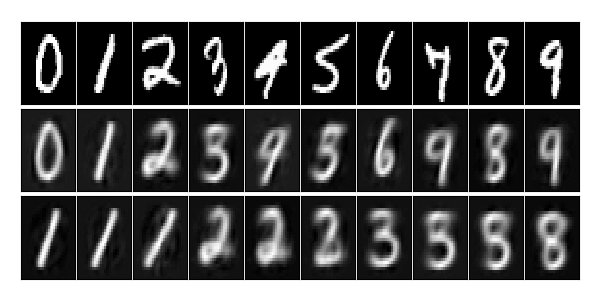
\includegraphics[scale=0.8]{data/chapter_survey/mnist_reconstruction_generation}\caption{Example of a simple VAE trained on the MNIST dataset. Here, the neural networks modelling the encoder and decoder parameters contained two levels of convolutional blocks. Ground truth examples are in the top row, reconstructed samples are in the middle row, artificially generated digits are in the bottom row. The reconstructions are blurry, which is a typical VAE behaviour. Also, the reconstruction is imperfect for digits which resemble each other, such as "9", "4" and "7", or "3" and "8". The artificial digits were created by linearly interpolating between two coordinates in the latent space and using this as an input to the decoder. The VAE then produces a smooth interpolation between digits "1" and "8" that contains the related digits "2" and "3".}
\label{fig:mnist_reconstruction}
\end{figure}
 
\subsubsection{Some VAE properties}
\begin{figure}
\begin{centering}
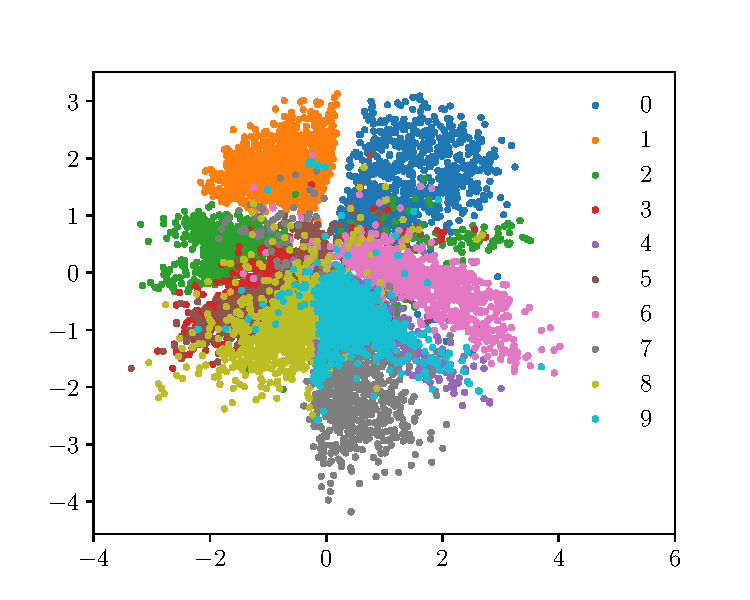
\includegraphics[scale=0.8]{data/chapter_survey/mnist_latent}
\par\end{centering}
\caption{The latent space of the MNIST dataset produced by a VAE with a two-dimensional latent space. Note the overlapping of some digit encodings, e.g. "7" and "9".}
\label{fig:mnist_latent}
\end{figure}

If a VAE model is correctly trained, we can assume that the encoder $q_{\vc{\phi}}(\vc{z}|\vc{x})$ and prior $p(\vc{z})=\mathcal{N}(\vc{z}|0,\textbf{I})$ are close to each other. Then, samples from the prior can be fed to the decoder and one can expect artificial samples that resemble the training data. A \textbf{generated sample} can therefore be described as
\begin{equation} \label{eq:generated_sample}
    \tilde{\vc{x}} = \vc{\mu}_{\vc{\theta}}(\vc{z}), \vc{z} \sim p(\vc{z}).
\end{equation}
Note that a \textbf{reconstructed sample} is instead obtained by sampling the encoding $\vc{z}$ from the encoder through the reparametrization trick~\eqref{eq:vae_reparam}. This is also a place to note why we are using neural network representation of the encoder and decoder. Since neural networks have be proven to be universal function approximators, we know that given enough capacity, data and training time, the decoder can learn a mapping from the prior to an arbitrary function.

\begin{figure}
\centering
    \begin{subfigure}[b]{0.45\textwidth}
        \centering
        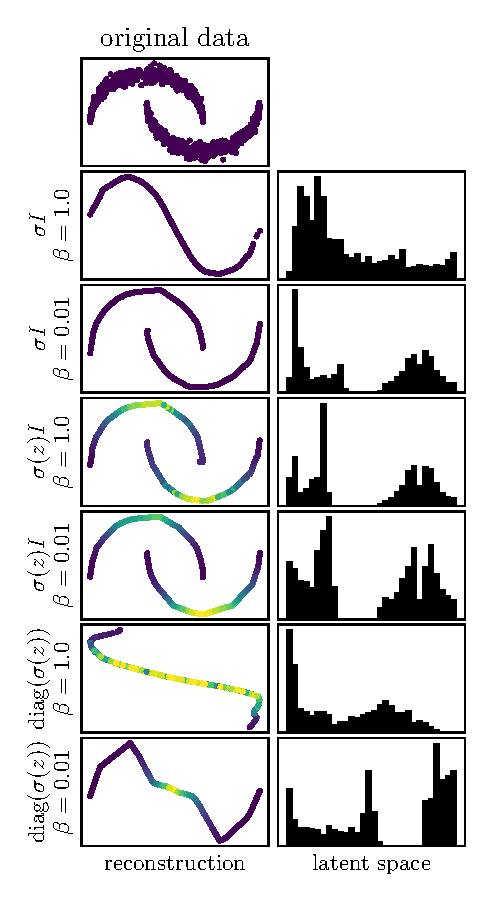
\includegraphics[scale=0.9]{data/chapter_survey/vae_two_moons_z1_colored}
        \caption{$h=1$}
    \end{subfigure}
    \begin{subfigure}[b]{0.45\textwidth}
        \centering
        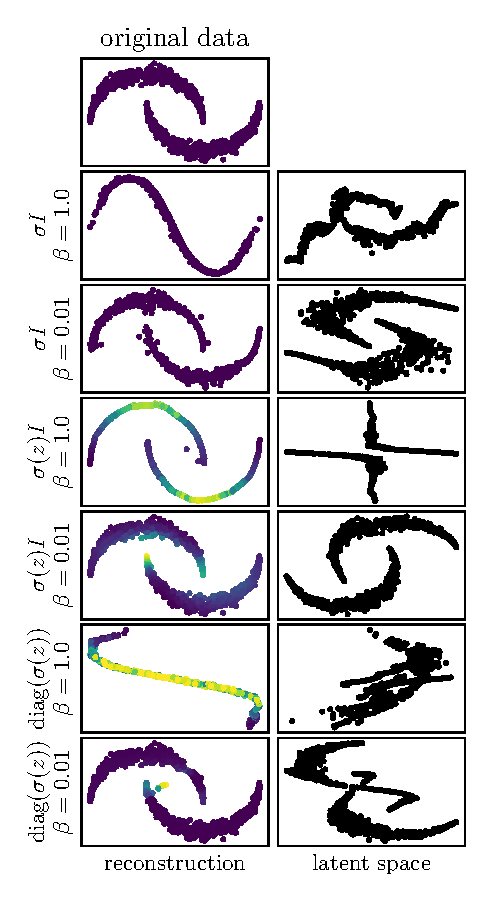
\includegraphics[scale=0.9]{data/chapter_survey/vae_two_moons_z2_colored}
        \caption{$h=2$}
    \end{subfigure}
\caption{An overview of VAE behaviour with respect to the scaling parameter $\beta$ of the objective~\eqref{eq:betavae} and to the way the covariance of the decoder $p_{\vc{\theta}}(\vc{x}|\vc{z})$ is estimated. The VAE model was trained on the two--moons data, plotted in the plots at the very top. Variants with 1D (a) and 2D (b) latent spaces are compared, means of the decoder $\vc{\mu}_{\vc{\theta}}(\vc{z})$ are plotted on the left and the latent representations on the right. Clearly, smaller values of $\beta$ lead to better sample reconstruction, especially in the case of a two-dimensional latent space, as well as leading to a better separation of the encodings. This is understandable, since the prior $p(\vc{z})=\mathcal{N}(0,\textbf{I})$ is unimodal. From the top: the covariance of the decoder is given either by a fixed scalar ($\sigma I,\sigma=1$), by a scalar estimated from the data ($\sigma(\vc{z})I$), or by an estimate of its diagonal terms ($\text{diag}(\sigma(\vc{z}))$). The magnitude of the estimated variance in the two latter cases is denoted by color, where a brighter color corresponds to a higher value of variance. It is interesting that the second case ($\sigma(\vc{z})I$) seems to alleviate the reconstruction difficulties with higher $\beta$, while the estimation of the full covariance diagonal does not exhibit such property. Also, the third case seems to "exploit" the estimation of variance. Instead of pushing and optimizing the mean, it can instead simply put higher variance in the direction in which the reconstruction is worse and still incur only a small loss. Due to this behaviour, the second case seems to be the most robust and stable way of estimation of the reconstruction variance. Not surprisingly, the 2D case provides better reconstructions since it was provided with one more dimension to encode data to.}
\label{fig:betavae}
\end{figure}

Fig.~\ref{fig:mnist_latent} shows the latent space of an example VAE model. Note that although the overall distribution of the encodings resembles the normal prior, in order to be able to reconstruct the samples from the encodings, the model has to learn to encode the samples from different digit classes to different parts of the latent space. It was shown~\cite{higgins2017beta} that the reconstruction and regularization parts of the VAE loss~\eqref{eq:elbo3} actually work against each other. A model with encoder perfectly copying the randomness of the prior would not be able to reconstruct the inputs. On the other hand, a model without the latent regularization would not be able to generate new samples, as it would be practically identical with an AE model from Sec.~\ref{sec:reconstruction_models}, which is free to encode the different classes to arbitrary parts of the latent space. The basic loss~\eqref{eq:vae_loss} leads to a model that is usually in an equilibrium between both of these states. It is however possible to push the model in one of these directions by using a scaling parameter
\begin{equation} \label{eq:betavae}
\mathcal{L}_{\beta\text{VAE}}(\vc{x},\vc{\phi},\vc{\theta},\beta)= - \mathbb{E}_{q_{\vc{\phi}}(\vc{z}|\vc{x})}\left[\ln p_{\vc{\theta}}(\vc{x}|\vc{z})\right] + \beta D_{\text{KL}}\left(q_{\vc{\phi}}(\vc{z}|\vc{x})||p(\vc{z})\right),\beta>0.
\end{equation}
A VAE model trained with this loss is known as \textbf{BetaVAE}~\cite{higgins2017beta} and is one of the first VAE-based models that attempt some sort of \textbf{unsupervised disentanglement}. A disentangled model captures the possible factors of variation of a dataset in orthogonal dimensions of the latent space. Imagine a colored MNIST dataset, on which a disentangled model with a two dimensional latent space is trained. If properly disentangled, one latent dimension would capture the identity of the digit, while the other one would capture its color. This concept will be again revisited in Chapter~\ref{sec:chapter_sgvaegan}. The influence of the $\beta$ parameter is discussed in Fig.~\ref{fig:betavae}.

Instead of setting a fixed variance parameter $\sigma$ in the decoder, one can optimize and extract it instead from the last layer of the decoder, either as a scalar $\sigma_{\vc{\theta}}(\vc{z}) \in \mathbb{R}$
or even a full diagonal of the covariance $\text{diag}\left(\vc{\sigma}_{\vc{\theta}}(\vc{z})\right),\vc{\sigma}(\vc{z})\in\mathbb{R}^{d}$. From the experiment in Fig.~\ref{fig:betavae}, it seems (at least for tabular data) that the best results were surprisingly obtained not by the most complex variant, but the one with a scalar value $\sigma_{\vc{\theta}}$ optimized during training.

\subsection{Wasserstein and adversarial autoencoders}
The asymmetry of the KL divergence motivated search for a more accurate metric measuring the distance between the prior and the encoder. An alternative approach to VAE has been published in~\cite{mescheder2017adversarial} and improved in~\cite{tolstikhin2017wasserstein}, which proposes a general form of a generative autoencoder that uses a Wasserstein metric~\cite{givens1984class}. Unlike the KL divergence term in the VAE loss, which forces all the input data samples to zero (the mean of the standard prior), in \textbf{Wasserstein autoencoders} (WAE) the encoding is loosened, which reportedly leads to improved reconstruction~\cite{tolstikhin2017wasserstein}. A general form of the loss function of a WAE model is
\begin{equation} \label{eq:general_wae_loss}
    \mathcal{L}_{\text{WAE}} (\vc{x}, \vc{\theta}, \vc{\phi}) = - \mathbb{E}_{q_{\vc{\phi}}(\vc{z}|\vc{x})} \left[ \log p_{\vc{\theta}}(\vc{x}|\vc{z}) \right] + \lambda D_{\text{W}} \left( q_{\vc{\phi}}(\vc{z}|\vc{x}) || p(\vc{z}) \right),
\end{equation}
where $\lambda >0$  is a scalar hyperparameter, and $D_{\text{W}}$ is a Wasserstein metric. The most commonly used form of the Wasserstein metric is the kernelized \textbf{maximum-mean-discrepancy} (MMD) with a kernel function $k_f:\mathbb{R}^d \times \mathbb{R}^d \rightarrow \mathbb{R}$, which was reported to perform well in matching high dimensional distributions~\cite{zhao2017infovae}. From the theoretical point of view, KLD only matches the first and the second moment of the two distributions, while MMD can potentially match an infinite amount of moments with the right kernel. Some authors~\cite{tolstikhin2017wasserstein} argue that by minimizing KLD, the latent representation might become uninformative for the decoder to reconstruct the code. On the other hand, MMD maximizes the mutual information between $\vc{x}$  and $\vc{z}$~\cite{zhao2017infovae}.

Under some mild assumptions about the kernel function $k_f$ (see details in~\cite{tolstikhin2017wasserstein}) the MMD can be expressed in such a way that enables optimization of the model by backpropagation. Then, the MMD of the prior and the encoder can be approximated solely by comparing sets of samples from these  distributions $Z_q=\{\vc{z}_{q,1}, \vc{z}_{q,2}, \ldots, \vc{z}_{q,n}\}, Z_p=\{\vc{z}_{p,1}, \vc{y}_{p,2}, \ldots, \vc{y}_{p,n}\},\vc{z}_{q,i}\sim q_{\vc{\phi}}(\vc{z}|\vc{x}),\vc{z}_{p,i} \sim p(\vc{z}),\forall i \in \hat{n}$ in a closed expression
\begin{equation} \label{eq:mmd}
\text{MMD}_{k}(Z_p,Z_q)=\frac{1}{n(n-1)}\sum_{i\neq j}k_f(\vc{z}_{q,i},\vc{z}_{q,j})+\frac{1}{n(n-1)}\sum_{i\neq j}k_f(\vc{z}_{p,i},\vc{z}_{p,j})-\frac{2}{n^{2}}\sum_{i,j}k_f(\vc{z}_{q,i}, \vc{z}_{p,j}).
\end{equation}
The most notable characteristic of the MMD is that in practice, it only require samples from the distributions in question, and it is therefore less restricting than the KLD, which required normal prior and encoder in order to obtain the analytic expression~\eqref{eq:vae_kld}. This offers the potential for the use of a variety of prior and encoder distributions. The two most common choices of $k_f$ are the RBF $k_f(x,y) = \exp(- \gamma \vert \vert x - y \vert \vert_2^2), \gamma > 0$ and inverse multiquadratics (IMQ) $k_f(x,y) = (c^2 +  \vert \vert x - y \vert \vert_2^2)^\beta, c>0, \beta < 0$ kernels. The training algorithm for a Wasserstein autoencoder with the MMD loss is in Alg.~\ref{alg:infovae}. Note that although the parameters $\vc{\phi}$ do not appear directly in the loss on line 7 of the algorithm, they are present through the samples $\tilde{Z_{L}}$. 

\begin{algorithm}
\begin{algorithmic}[1]
\Require{A WAE model with encoder $q_{\vc{\phi}}(\vc{z}|\vc{x})$, decoder $p_{\vc{\theta}}(\vc{x}|\vc{z})$ and a prior $p(\vc{z})$, training set $X=\lbrace \vc{x}_1, \vc{x}_2, \ldots, \vc{x}_n \rbrace \subset \mathcal{X}$, maximum number of iterations $I\in\mathbb{N}$, batchsize $B \in \mathbb{N}$, regularization coefficient $\lambda > 0$, characteristic positive definite kernel $k_f$, standard deviation parameter $\sigma$ > 0.}
\State $\vc{\phi},\vc{\theta} \gets $ Initialize parameters
\State{$i \gets $ Iteration counter}
\While{$i<I$ or $\vc{\phi},\vc{\theta}$ are not converged}
	\State{$X_B \gets$ A random batch of $B$ samples from $X$}
	\State{$Z \gets \lbrace \vc{z}_j \sim q_{\phi}(\vc{z}|\vc{x}_j), \vc{x}_j \in X_B \rbrace$ samples from the encoder}
	\State{$\tilde{Z} \gets$ A random batch of $B$ samples from prior $p(\vc{z})$}
	\State$l \gets \frac{1}{B}\sum_{j=1}^B  ||\vc{x}_j-\vc{\mu}_{\vc{\theta}}(\vc{z}_j)||_{2}^{2} +\lambda \text{MMD}_k(Z,\tilde{Z}), \vc{x}_j \in X_B, \vc{z}_j \in Z$
	\State$\vc{\phi} \stackrel{+}\gets - \nabla_{\vc{\phi}}l $ update of encoder weights
	\State$\vc{\theta} \stackrel{+}\gets - \nabla_{\vc{\theta}}l $ update of decoder weights
	\State{$i \gets i+1$}
\EndWhile
\State{\textbf{return} encoder $q_{\vc{\phi}}(\vc{z}|\vc{x})$, decoder $p_{\vc{\theta}}(\vc{x}|\vc{z})$}
\end{algorithmic}

\caption{InfoVAE training procedure.}
\label{alg:infovae}
\end{algorithm}



\subsection{Adversarial Autoencoder}

A different architecture arises when the Jensen--Shannon divergence
$D_{\text{JS}}$ is used in place of $D_{Z}$. The JS divergence is
a symmetrical (unlike KL divergence) measure of distance between two
probability distributions. The use of $D_{\text{JS}}$ leads to a
model that is called adversarial autoencoder (AAE) and was originally
proposed in~\cite{makhzani2015adversarial}. It was shown in~\cite{tolstikhin2017wasserstein}
how the use of $D_{\text{JS}}$ leads to the use of GAN loss that
was described in the previous part. To regularize the encoder, we
add a discriminator $d_{\eta}(\vc{z}):\mathcal{Z}\rightarrow\left[0,1\right]$
represented by a neural network with parameters $\eta$. The discriminator
has the same function as the one in the GAN model -- it tries to
recognize latent space samples produced by the encoder and those sampled
from the prior $p(\vc{z})$. The difference is that the discriminator now
operates on the latent space $\mathcal{Z}$ instead of the data space
$\mathcal{X}$. 

\begin{figure}
\centering{}\begin{tikzpicture}
  \node[const]                               (x) {$\vc{x}$};
  \node[const, right = 0.3cm of x]           (xin) {};
  % encoder in
  \node[latent, right = 0.4cm of x, yshift = 0.825cm] (E11) {};
  \node[latent, right = 0.4cm of x, yshift = 0.275cm] (E12) {};
  \node[latent, right = 0.4cm of x, yshift = -0.275cm] (E13) {};
  \node[latent, right = 0.4cm of x, yshift = -0.825cm] (E14) {};
  % encoder hidden
  \node[latent, right = 1.6cm of x, yshift = 0.55cm] (E21) {};
  \node[latent, right = 1.6cm of x, yshift = 0cm] (E22) {};
  \node[latent, right = 1.6cm of x, yshift = -0.55cm] (E23) {};
  % encoder out
  \node[latent, right = 2.8cm of x, yshift = 0.275cm] (E31) {};
  \node[latent, right = 2.8cm of x, yshift = -0.275cm] (E32) {};
  % encoder tag
  \node[const, right = 1.4cm of x, yshift = 1.1cm] (E) {$q_{\vc{\phi}}(\vc{z}|\vc{x})$};
  % placement
  \node[const, right = 5.2cm of x, yshift=1.2cm]           (encoderin) {}; 
  \node[const, right = 5.2cm of x, yshift=-1.2cm]           (discriminatorin) {}; 
  % code
  \node[const, right = 4.1cm of x, yshift = 0cm]           (zg) {$\vc{z}$};
  \node[const, right = 3.4cm of x]           (zgout) {}; 
  \node[const, right = 0cm of encoderin]           (zgin) {};
  \node[const, right = 0.05cm of zg]           (zgout2) {};
  \node[const, right = 0cm of discriminatorin,yshift=0.05cm]           (zgin2) {};
  % prior
  \node[const, right = -1.8cm of discriminatorin, yshift = 0cm]         (z) {$\tilde{\vc{z}} \sim p(\vc{z})$};
  \node[const, right = 0cm of z, yshift = 0cm]         (zout) {};
  \node[const, right = 0cm of discriminatorin]           (zin) {};

  % decoder in
  \node[latent, right = 0.1cm of encoderin, yshift = 0.275cm] (D11) {};
  \node[latent, right = 0.1cm of encoderin, yshift = -0.275cm] (D12) {};
  % decoder hidden
  \node[latent, right = 1.3cm of encoderin, yshift = 0.55cm] (D21) {};
  \node[latent, right = 1.3cm of encoderin, yshift = 0cm] (D22) {};
  \node[latent, right = 1.3cm of encoderin, yshift = -0.55cm] (D23) {};
  % decoder out
  \node[latent, right = 2.5cm of encoderin, yshift = 0.825cm] (D31) {};
  \node[latent, right = 2.5cm of encoderin, yshift = 0.275cm] (D32) {};
  \node[latent, right = 2.5cm of encoderin, yshift = -0.275cm] (D33) {};
  \node[latent, right = 2.5cm of encoderin, yshift = -0.825cm] (D34) {};
  % xhat
  \node[const, right = 3.4cm of encoderin]           (xhat) {$\vc{x}'$};
  \node[const, right = -0.8cm of xhat]       (xhatout) {};    
  % decoder tag
  \node[const, right = 1.1cm of encoderin, yshift = 1.1cm] (D) {$p_{\vc{\theta}}(\vc{x}|\vc{z})$};   
  
  % discriminator
  \node[latent, right = 0.1cm of discriminatorin, yshift = 0.275cm] (DI11) {};
  \node[latent, right = 0.1cm of discriminatorin, yshift = -0.275cm] (DI12) {};
  % discriminator hidden
  \node[latent, right = 1.3cm of discriminatorin, yshift = 0.55cm] (DI21) {};
  \node[latent, right = 1.3cm of discriminatorin, yshift = 0cm] (DI22) {};
  \node[latent, right = 1.3cm of discriminatorin, yshift = -0.55cm] (DI23) {};
  % discriminator out
  \node[latent, right = 2.5cm of discriminatorin, yshift = 0cm] (DI31) {};
  % xhat
  \node[const, right = 3.45cm of discriminatorin]           (dx) {$s \in [0,1]$};
  \node[const, right = -1.9cm of dx]       (dxout) {};       
  % discriminator tag
  \node[const, right = 1.1cm of discriminatorin, yshift = 1.1cm] (D) {$d_{\vc{\eta}}(\vc{z})$};

  % edges
  \nedge {x} {xin}
  % encoder 
  \nedge {E11, E12, E13, E14} {E21, E22, E23}
  \nedge {E21, E22, E23} {E31, E32}
  % latent
  \nedge {zgout} {zg}
  \nedge {zgout2} {zgin}
  \nedge {zgout2} {zgin2}
  \nedge {zout} {zin}

  % decoder
  \nedge {D11, D12} {D21, D22, D23}
  \nedge {D21, D22, D23} {D31, D32, D33, D34} 
  % discriminator
  \nedge {DI11, DI12} {DI21, DI22, DI23}
  \nedge {DI21, DI22, DI23} {DI31}
  %xhat
  \nedge {xhatout} {xhat}
  %xhat
  \nedge {dxout} {dx}

\end{tikzpicture}
\caption{A schematic of a AAE model consisting of fully connected layers. A
data sample $x$ is mapped to latent space representation $\tilde{z}$
via the encoder $q_{\vc{\phi}}(\vc{z}|x)$. Also, a sample $z$ is sampled from
the latent prior $p(\vc{z})$. Both $z$ and $\tilde{z}$ are passed to
the discriminator $d_{\eta}(\vc{z})$ that produces a score $s$ -- the
probability that the input sample comes from the latent prior. At
the same time, the latent representation is passed to the decoder
$p_{\vc{\theta}}(x|z)$ which maps it to a reconstruction $\tilde{x}$.}
\label{fig:aae}
\end{figure}

The GAN loss function~(\ref{eq:disc_loss}) is used to train the
discriminator, while the loss function~(\ref{eq:gen_loss}) is added
to the reconstruction term for training of the encoder and decoder.
The AAE training losses to be maximized are then
\begin{equation}
\mathcal{L}_{d}(\vc{z},\tilde{z},\eta)=\ln d_{\eta}(\vc{z})+\ln(1-d_{\eta}(\tilde{z})),\label{eq:aae_loss_disc}
\end{equation}
\begin{equation}
\mathcal{L}_{ae}(x,\tilde{x},\tilde{z},\vc{\theta},\vc{\phi})=c(x,\tilde{x})-\lambda\ln d_{\eta}(\tilde{z}),\label{eq:aae_loss_autoencoder}
\end{equation}
where $\lambda>0$, $z\sim p(\vc{z})$, $x\sim p(x)$, $\tilde{z}\sim q_{\vc{\phi}}(\vc{z}|x)$
and $\tilde{x}\sim p_{\vc{\theta}}(x|\tilde{z})$.

\begin{algorithm}
\begin{algorithmic}[1]
\Require{An AAE model with encoder $q_{\vc{\phi}}(\vc{z}|\vc{x})$, decoder $p_{\vc{\theta}}(\vc{x}|\vc{z})$,  a prior $p(\vc{z})$ and a discriminator $d_{\vc{\eta}}(\vc{z})$, training set $X=\lbrace \vc{x}_1, \vc{x}_2, \ldots, \vc{x}_n \rbrace \subset \mathcal{X}$, maximum number of iterations $I\in\mathbb{N}$, batchsize $B \in \mathbb{N}$, regularization coefficient $\lambda > 0$, standard deviation parameter $\sigma$ > 0.}
\State $\vc{\phi},\vc{\theta}, \vc{\eta} \gets $ Initialize parameters
\State{$i \gets $ Iteration counter}
\While{$i<I$ or $\vc{\phi},\vc{\theta},\vc{\eta}$ are not converged}
	\State{$X_B \gets$ A random batch of $B$ samples from $X$}
	\State{$Z \gets \lbrace \vc{z}_j \sim q_{\vc{\phi}}(\vc{z}|\vc{x}_j), \vc{x}_j \in X_B \rbrace$ samples from the encoder}
	\State{$\tilde{Z} \gets$ A random batch of $B$ samples from prior $p(\vc{z})$}
	\State{$\tilde{X} \gets \lbrace\tilde{\vc{x}}_j \sim p_{\vc{\theta}}(\vc{x}|\tilde{\vc{z}}_j), \tilde{\vc{z}}_j \in \tilde{Z}_B \rbrace$ generated samples}
	\State$l_{ae} \gets \frac{1}{B}\sum_{j=1}^B \mathcal{L}_{\text{AAE}}( \vc{x}_j,\vc{z}_j,\tilde{\vc{z}}_j, , \vc{\theta}, \vc{\phi} ) , x_j \in X_B, \vc{z}_j \in Z, \tilde{\vc{z}}_j \in \tilde{Z}$
	\State{$l_d \gets \frac{1}{B}\sum_{j=1}^B \mathcal{L}_{\text{AAE}_d}(\vc{z}_j,\tilde{\vc{z}}_j, \vc{\eta}), \vc{z}_j \in Z, \tilde{\vc{z}}_j \in \tilde{Z}$}
	\State$\vc{\phi} \stackrel{+}\gets - \nabla_{\vc{\phi}}l_{ae} $ update of encoder weights
	\State$\vc{\theta} \stackrel{+}\gets - \nabla_{\vc{\theta}}l_{ae} $ update of decoder weights
	\State$\vc{\eta} \stackrel{+}\gets - \nabla_{\vc{\eta}}l_{d} $ update of discriminator weights
	\State{$i \gets i+1$}
\EndWhile
\State{\textbf{return} encoder $q_{\vc{\phi}}(\vc{z}|\vc{x})$, decoder $p_{\vc{\theta}}(\vc{x}|\vc{z})$, discriminator $d_{\vc{\eta}}(\vc{z})$}
\end{algorithmic}

\caption{AAE training procedure.}
\label{alg:aae}
\end{algorithm}

The AAE training procedure is described in Alg.~\ref{alg:aae}.
Again, any prior $p(\vc{z})$ that we can sample from is suitable for the
regularization of AAE, even a multimodal one. A schematic of the AAE
model is in Fig.~\ref{fig:aae}. In practice, an AAE model compared
to InfoVAE behaves similarly as GAN compared to VAE. The adversarial
loss leads to less blurry reconstructions and generated samples at
the cost of higher training instability~\cite{tolstikhin2017wasserstein}.
One way to gain advantages of both is to use an AAE model as depicted
in Fig.~\ref{fig:aae} and add the MMD regularization term~(\ref{eq:mmd})
to the loss~(\ref{eq:aae_loss_autoencoder}).













As was already demonstrated, a common criticism of the VAE model is its use of the unit normal prior $p(\vc{z})$ which stimulates the distribution $q_{\vc{\phi}}(\vc{z}|\vc{x})$ to have a single mode, and therefore it is hard to fit data with a multi-modal latent distribution. The publication~\cite{tomczak2018vae} proposes a learnable multimodal \textbf{Vamp} prior realized as a mixture of $K \in \mathbb{N}$ independent Gaussian components. However, the Vamp prior is not compatible with the basic VAE model since its use does not lead to an analytical expression of KLD~\eqref{eq:vae_kld}. In the following text, we will describe alternatives to KLD regularization that are viable with this kind of prior. Then, the parameters of the components of the mixture are learned together with the parameters of the model.

\subsection{VAE in anomaly detection}
From the anomaly detection perspective, the basic criterion that test whether an input $\vc{x}$ is from the training (normal) data distribution is based on an estimate of the log-likelihood $- \ln p_{\vc{\theta}}(\vc{x}|\vc{z})$ is computed. However, using only the generating model with a prior
\begin{equation}
- \mathbb{E}_{p(\vc{z})}\left[\ln p_{\vc{\theta}}(x|z)\right]
\end{equation}
is theoretically well--justified, but it has been shown that this does not work well enough in practice~\cite{xu2018unsupervised}. Instead, the generative and discriminative distributions are used together to compute an estiamte of the \textbf{sampled reconstruction probability}
\begin{equation} \label{eq:rec_prob}
s_{\text{VAE}}(\vc{x})=-\frac{1}{L}\sum_{l=1}^{L}\ln p_{\vc{\theta}}(\vc{x}|\vc{z}^{l}) \approx-\mathbb{E}_{q_{\vc{\phi}}(\vc{z}|\vc{x})}\left[\ln p_{\vc{\theta}}(\vc{x}|\vc{z})\right].
\end{equation}
\begin{equation}
\vc{z}^l \sim q_{\vc{\phi}}(\vc{z}|\vc{x}) \nonumber 
\end{equation}
which was done in one of the first application of VAE in anomaly detection in~\cite{an2015variational}, where the authors successfully compare the VAE with AE and PCA on several anomaly datasets while claiming that the generative property of VAE can be used for causal analysis on the detected anomalies. Note that for a normal decoder, equation~(\ref{eq:vae_score}) is very similar to the reconstruction error of an  AE model~\eqref{eq:ae_objective}, with the difference that the reconstruction probability is computed from several samples of the encoder.

The reason for using the reconstruction probability of a VAE instead
of a reconstruction error of AE is the improved generalization that
was described in the previous section. It is discussed in~\cite{dai2017hidden}
that a VAE model is equivalent to a non--linear robust PCA model
and is proficient at dismissing sparse outliers. The authors also
make note of the fact that VAE is very efficient in pruning of unnecessary
latent dimensions in case when the real latent structure has lower
dimension than the chosen VAE latent space. However, sometimes~\cite{pereira2018unsupervised}
the reconstruction error of the VAE is used, which is defined as
\begin{equation}
f_{\text{VAEr}}(x)=-\frac{1}{M}\sum_{m=1}^{M}||x-\mathbb{E}\left[p_{\vc{\theta}}(x|z^{m}(\varepsilon)\right]||_{2}^{2},
\end{equation}
where only the mean of the generative distribution is compared to
the original sample $x$.

Another way of using VAE and other autoencoding models for anomaly
detection is to employ their ability to produce a low--dimensional
representation of high--dimensional data that preserves the important
relations between individual datapoints. Then, an anomaly detection
model (be it a generative or a classical one) can be trained on the
data encoded in the latent space. This two stage approach is especially
useful when the problem is in the image domain and some kind of vectorization
has to be used anyway. Also it enables the combination of countless
different approaches. Usage of this technique will be demonstrated
in one of the next chapters. It is also used in~\cite{dai2019diagnosing},
where both stages are a VAE and the second stage has the same input
and latent space dimensionality (therefore it does not compress data
at all). Although this paper does not present an application in anomaly
detection, it shows an improvement in learning of the latent space
prior. 

In~\cite{xu2018unsupervised} the authors present a so-called DonutVAE
with an enhanced loss function to detect anomalies in times series
data. The architecture is similar to that of a vanilla VAE, but the
loss becomes
\begin{equation}
\mathcal{L}_{\text{DVAE}}(x,\vc{\phi},\vc{\theta})=\mathbb{E}_{q_{\vc{\phi}}(\vc{z}|x)}\left[\beta\ln p(\vc{z})-\ln q_{\vc{\phi}}(\vc{z}|x)+\sum_{t=i}^{T}\alpha_{t}\ln p_{\vc{\theta}}(x|z)\right],\label{eq:donutvae}
\end{equation}
where $x=\{x_{t}\}_{t=1}^{T}$ is a sliding window of the last $T$
observations. Also, $\alpha_{t}=0$ if $x_{t}$ is anomalous or missing
and $\alpha_{t}=1$ otherwise and $\beta=\sum_{t=1}^{T}\alpha_{t}/T$.
The authors then show that usage of this loss function improves overall
results. This however has a caveat -- known anomalous samples must
be available, otherwise the loss~(\ref{eq:donutvae}) is the same
as~(\ref{eq:elbo2}). Furthermore, the authors claim that using
reconstruction probability~(\ref{eq:vae_score}) can be seen as
a weighted kernel density estimate.

The authors of~\cite{zong2018deep} couple an ordinary autoencoder
with a Gaussian mixture model (GMM) represented by a neural network.
The AE reduces the problem dimension to help overcome the curse of
dimensionality, while the GMM model serves as a density estimate in
the latent space. The novelty of the method is in two facts. Firstly,
instead of training parameters of both models separately, they are
learnt jointly which improves the performance of the model. Secondly,
the input of the GMM model is not only the latent representation,
but also the reconstruction error of the sample. The loss is 
\begin{eqnarray}
\mathcal{L}_{\text{DAGMM}}(x,\vc{\phi},\vc{\theta},\omega) & = & ||x-d_{\vc{\theta}}(e_{\vc{\phi}}(x))||_{2}^{2}+\lambda_{1}E_{\omega}(\vc{z})+\lambda_{2}P(\hat{\Sigma)}\\
z & = & \left[e_{\vc{\phi}}(x),||x-d_{\vc{\theta}}(\vc{z})||_{2}^{2}\right]^{T}\\
E_{\omega}(\vc{z}) & = & -\ln\left(\sum_{i=1}^{d}\pi_{\omega,i}\frac{\exp\left(-\frac{1}{2}(\vc{z}-\mu_{\omega,i})^{T}\Sigma_{i}^{-1}(\vc{z}-\mu_{\omega,i})\right)}{\sqrt{|2\pi\Sigma_{\omega,i}|}}\right)
\end{eqnarray}
where we recognize the reconstruction error of the AE, the energy
term $E_{\omega}(\vc{z})$ of the GMM model and a penalization $P(\Sigma)$
that prevents the covariance matrices in the GMM model to become singular,
$\lambda_{1},\lambda_{2}>0$ are scaling parameters. Parameters $\left\{ \pi_{\omega,i},\mu_{\omega,i},\Sigma_{\omega,i}\right\} _{i=1}^{d}$
are the parameters of the GMM model estimated by a neural network
with weights $\omega$. The sample energy is used as anomaly score.
Although this model is not based on VAE, we can view the energy term
as being similar to the KL divergence term in the VAE loss as it also
imposes some kind of structure in the latent space.

A VAE model couple with an LSTM recurrent neural network with attention
mechanism is used in~\cite{pereira2018unsupervised} for detecting
anomalies in time series. They operate in the semisupervised setting,
where only labeled normal samples are used for training. Although
the authors share some interesting insights, e.g. that the VAE is
able to capture the temporal structure in the data, they do not offer
a thorough comparison with other methods.




\subsection{Wasserstein autoencoders in anomaly detection}

For InfoVAE, the anomaly score can be either the reconstruction error~(\ref{eq:ae_score})
or the reconstruction probability~(\ref{eq:vae_score}) depending
on whether a deterministic or a stochastic decoder is used. In the
AAE model, we can use the loss of a trained model which combines the
reconstruction error term with the discriminator score 
\begin{equation}
f_{\text{AAE}}(x)=\mathcal{L}_{ae}(x,\tilde{x},\tilde{z},\bar{\vc{\theta}},\bar{\vc{\phi}}),\tilde{z}\sim q_{\bar{\vc{\phi}}}(\vc{z}|x),\tilde{x}\sim p_{\bar{\vc{\theta}}}(x|\tilde{z}),\label{eq:aae_score}
\end{equation}
where $\bar{\vc{\theta}},\bar{\vc{\phi}}$ are fixed parameters of the trained
neural network. This anomaly score has one tuning hyperparameter $\lambda$
which governs how much the information from the discriminator weighs
in to the decision. As said before, the reconstruction term $c(x,\tilde{x})$
is either a reconstruction error or probability based on the type
of decoder.

The AAE model is used in~\cite{leveau2017adversarial} where it
is benchmarked on the MNIST problem. Standard distribution is compared
to a Gaussian mixture model (GMM) when used as priors $p(\vc{z})$ and
a special rejection component is introduced for representation of
anomalies. 

In~\cite{chen2018unsupervised} an AAE model is compared to the
VAE model on the task of detection of brain abnormalities in MRI images.
The loss function of the autoencoding part is enhanced by a term $\alpha||z-z^{\prime}||$,
where $z$ is a the latent representation of a sample $x$ and $z'$
is the latent representation of the reconstructed sample $\tilde{x}$.
This is supposed to improve consistency of the representation. The
thesis~\cite{dimokranitou2017adversarial} also uses AAEs for detection
of abnormalities in videos. The model presented in~\cite{pidhorskyi2018generative}
uses an additional discriminator on top of the decoder in AAE to improve
reconstruction and generative property. The model is then tested for
anomaly detection on standard benchmark datasets.

Clearly, some work has already been done in the area of AAE and anomaly
detection, but not a lot of authors use the InfoVAE model for this
specific task.


\subsection{Normalizing flows}
The name normalizing flows refers to methods relying on the change of variables formula
\begin{equation}
    p\left(\vec{x}\right) = p\left(\vec{z}\right)\!\left\vert \text{det} J_f\!\left(\vec{z}\right) \right\vert^{-1}, ~ \vec{z} = f^{-1}\!\left(\vec{x}\right),
\label{eq:rv_transformation}
\end{equation}
where $J_f\!\left(\vec{z}\right)$ is Jacobi matrix of function $f$ evaluated at $\vec{z}$. $p(\vec{z})$ is a known distribution of the latent variable $\vec{z}$ from space $\mathcal{Z}$ of the same dimension as $\mathcal{X}$.

Theoretical reviews~\cite{papamakariosNormalizingFlowsProbabilistic2019, kobyzevNormalizingFlowsIntroduction2020} require $f$ to be invertible and both $f$ and $f^{-1}$ to be differentiable. Therefore, flow models primarily differ in how they define the class of functions $f$, which ranges from simple affine transformations to solutions of ordinary differential equations. The expressive power comes from their composition, as is usual in neural networks. In the comparison, we consider flows on tabular data only, for which we have implemented the well-known RealNVP~\cite{dinh2016density} and MAF~\cite{papamakariosMaskedAutoregressiveFlow2018} flows alongside a promising class of Sum-Product-Transform networks --- SPTN~\cite{pevny2020sum} combining normalizing flows with a graphical model. The likelihood is used as a natural anomaly score.

Flow models have not yet enjoyed much popularity in anomaly detection~\cite{yamaguchi2019adaflow, schmidtNormalizingFlowsNovelty2019, diasAnomalyDetectionTrajectory2020a, pevny2020sum} in comparison to the autoencoder-based models reviewed below. To us, this is surprising since these methods can exactly calculate likelihood functions, which under a good fit are the ideal anomaly score. Meanwhile, the focus of the surrounding community is on the topic of \textit{out of distribution detection} (OOD)\footnote{Out of distribution detection means identifying samples coming from a different dataset. For example, a model trained on MNIST / CIFAR10 should assign a low likelihood to samples from Fashion MNIST / SVHN respectively.}~\cite{nalisnickDeepGenerativeModels2019}, which is very related to anomaly detection if not being equal. Ref.~\cite{choiWAICWhyGenerative2019} suggests to use ensembles, while~\cite{renLikelihoodRatiosOutofDistribution2019} recommends to convert the single-class problem to classification problems in the spirit of \cite{steinwart2005a}. A deep investigation of OOD in~\cite{kirichenkoWhyNormalizingFlows2020} shows that with low-level features such as pixel intensities, flows tend to learn local models, i.e. according to taxonomy in~\cite{ruff2020unifying} they fail to detect semantic anomalies.


TODO:

\begin{itemize}
    \item read through the generativead paper and see if we are missing any models here
    \item also compare the scores etc.
\end{itemize}